
\documentclass[a4paper,11pt]{article}


%%% fontenc
%\usepackage{fontspec,xunicode,xltxtra}
%\setmainfont{Times New Roman}
%\setsansfont{Source Sans Pro}
%\setmonofont{Source Sans Pro}

%%% xeCJK
\usepackage{xeCJK}
\setCJKmainfont[BoldFont=Adobe Heiti Std]{Adobe Song Std}
\setCJKsansfont[BoldFont=Adobe Heiti Std]{Adobe Song Std}
\setCJKmonofont[BoldFont=Adobe Heiti Std]{Adobe Song Std}
\XeTeXlinebreaklocale "zh"
\XeTeXlinebreakskip=0pt plus 1pt minus 0.1pt

\usepackage{xcolor}
\usepackage{graphicx}

%%% get total page number
\usepackage{lastpage}

%%% customized definition
\makeatletter
\def\sybtitle#1{\def\@sybtitle{#1}}
\def\sybauthor#1{\def\@sybauthor{#1}}
\def\sybdate#1{\def\@sybdate{#1}}
\sybtitle{}
\sybauthor{}
\sybdate{}
\def\sybmaketitle{
  \begin{center}
  \vspace*{.8in}
  {\huge\bfseries\@sybtitle}
  \par
  \vspace{.8in}
  {\Large\@sybauthor}
  \par
  \vspace{.2in}
  \@sybdate
  \vspace{.5in}
  \end{center}
}
\makeatother
\setlength{\parindent}{0pt}
\renewcommand{\today}{\number\month 月 \number\day 日, ~\number\year 年}
\def\lt{\textless}
\def\gt{\textgreater}
\renewcommand\contentsname{\bfseries 目~~录}
\newcommand\bs{\texttt{\symbol{'134}}} % input backslash sign
%\newcommand\bs{\string\} % same as above definition
\long\def\cmd#1{\par\vspace{.5em}\hspace*{2em}#1\vspace{.5em}\par}
\def\cstr#1{\texttt{\string#1}} % e.g. \cstr{\latex}
\long\def\runcode#1{\par\bigskip#1\bigskip\par}
% 我不想看到那么多的underful hbox,尤其是minted环境加上背景色之后
\hbadness=10000
% 适当放宽overful hbox的限制,运行2pt的溢出
\hfuzz=2pt
\parskip=3\lineskip


%%% change background color & add frame for enumerate enviroment
\usepackage{mdframed}
\newmdenv[backgroundcolor=blue!10,linewidth=0pt]{coloredframe}
\newenvironment{coloredenumerate}{
  \begin{coloredframe}
  \begin{enumerate}
}{
  \end{enumerate}
  \end{coloredframe}
}

%%% geometry
\usepackage[includehead,includefoot,hmargin=21mm,vmargin=10.5mm,
            headsep=12pt,headheight=25pt]{geometry}
%\usepackage[includehead,includefoot,hmargin=1.2in,vmargin=1in]{geometry}

%%% fancyhdr
\usepackage{fancyhdr}
\makeatletter
\fancypagestyle{main} {
  \fancyhf{} % clear header & footer
  \fancyhead[L]{\bfseries\@sybtitle}
  \fancyhead[R]{\thepage/\pageref*{LastPage}}
  \renewcommand{\headrulewidth}{0.4pt} % header line
  \renewcommand{\footrulewidth}{0pt} % footer line
}
\fancypagestyle{header} {
  \fancyhf{} % clear header & footer
  \fancyfoot[C]{\roman{page}}
  \renewcommand{\headrulewidth}{0pt} % header line
  \renewcommand{\footrulewidth}{0pt} % footer line
}
\makeatother

\usepackage{titlesec}
\titleformat{\part}{\centering\Large\bfseries}{第\,\thepart\,部分}{1em}{}
\titleformat{\section}{\large\bfseries}{\thesection}{1em}{}
\titleformat{\subsection}{\normalsize\bfseries}{\thesubsection}{1em}{}
%\titlespacing*{章节命令}{左边距}{上文距}{下文距}[右边距]
\titlespacing*{\section}{0pt}{2\baselineskip}{\parsep}


\usepackage{hyperref}

%%% perfect source code display
\usepackage{minted}
%\usemintedstyle{colorful}
\definecolor{srcbg}{rgb}{0.95,0.95,0.95}
\newminted{java}{linenos,tabsize=4,bgcolor=srcbg}
\newminted{xml}{linenos,tabsize=4,bgcolor=srcbg}
\newminted{cpp}{linenos,tabsize=4,bgcolor=srcbg}
\newminted{bash}{linenos,tabsize=4,bgcolor=srcbg}
\newminted{latex}{linenos,tabsize=4,bgcolor=srcbg}



\usepackage{xcolor}
\colorlet{HEADCOLOR}{red!50}
\colorlet{BRANCHCOLOR}{blue!50}
\colorlet{WORKCOLOR}{gray!50}
\colorlet{INDEXCOLOR}{cyan!50}
\colorlet{COMMITCOLOR}{green}

\usepackage{tikz}
\usetikzlibrary{shapes,arrows,positioning,calc,backgrounds,matrix,fit,decorations.pathreplacing}
\tikzset{
  basic-style/.style = {
    rectangle, rounded corners=2pt, draw, thick,
    fill=#1,
    minimum height=15pt,
    minimum width=1.5cm,
    inner sep=1pt
  },
  commit-style/.style = {
    basic-style=COMMITCOLOR
  },
  index-style/.style = {
    basic-style=INDEXCOLOR,
    minimum width=2.5cm
  },
  work-style/.style = {
    basic-style=WORKCOLOR,
    minimum width=2.5cm
  },
  branch-style/.style = {
    basic-style=BRANCHCOLOR
  },
  head-style/.style = {
    basic-style=HEADCOLOR
  },
  cmd-style/.style = {
    #1=5pt
  },
  cmd-style/.default = right,
  main-style/.style = {
    execute at end picture = {
      \begin{pgfonlayer}{background}
        \path[fill=gray!20,rounded corners]
          ([xshift=-0.2cm,yshift=-0.2cm]current bounding box.south west) rectangle
          ([xshift=0.2cm,yshift=0.2cm]current bounding box.north east);
          %(current bounding box.south west) rectangle
          %  (current bounding box.north east);
        \end{pgfonlayer}
    }
  },
  file-style/.style = {
    draw=red, fill=yellow!30, inner sep=2pt
  },
  dir-style/.style = {
    fill=green!50,inner sep=2pt
  },
  dir-bg-style/.style = {
    fill=cyan!30,rounded corners
  },
  every edge/.style = {draw, ->, >=latex', thick}
}

%%%%% new definitions %%%%%

\newlength\commitDistance
\setlength\commitDistance{0.5cm}
\newlength\indexWorkDistance
\setlength\indexWorkDistance{2\commitDistance}

\newcommand\displayName[1]{\ttfamily\bfseries #1}
\newcommand\commandName[1]{\ttfamily\bfseries\small #1}

\def\createNode style:#1 name:#2 display:#3 direct:#4 distance:#5 to:#6;{
  \node [#1, #4=#5 of #6] (#2) {#3}
        edge [#4] (#6);
}
\def\createCommit name:#1 display:#2 direct:#3 to:#4;{
  \node [commit-style, #3=\commitDistance of #4] (#1) {#2}
        edge [#3, COMMITCOLOR] (#4);
}
\def\createBranch name:#1 display:#2 direct:#3 to:#4;{
  \node [branch-style, #3=0.75\commitDistance of #4] (#1) {#2}
        edge [#3, BRANCHCOLOR] (#4);
}
\def\createHead direct:#1 to:#2;{
  \node [head-style, #1=0cm of #2] (head) {\displayName HEAD};
}
\def\createIndex to:#1;{
  \node [index-style, below=2\commitDistance of #1] (index) {\displayName Index};
}
\def\createWork to:#1;{
  \node [work-style, below=2\commitDistance of #1] (work) {\displayName Work DIR};
}

\newcommand\makeOutline{
  %\useasboundingbox (-0.1,-3.6) rectangle (10.7,2);
  \node[right] (dumy) at (0,0) {\dots};
  \createCommit name:a display:{\displayName A} direct:right to:dumy;
  \createCommit name:b display:{\displayName B} direct:right to:a;
  \createCommit name:c display:{\displayName C} direct:right to:b;
  \createCommit name:d display:{\displayName D} direct:right to:c;
  \createCommit name:e display:{\displayName E} direct:right to:d;

  \createIndex to:c;
  \createWork to:index;
}

\newcommand\createMatrix[2]{
  \matrix [
    matrix of nodes,
    nodes={rectangle,draw=red,fill=yellow!30,minimum width=1.3cm,font=\ttfamily\small,inner sep=2pt},
    row sep=-\pgflinewidth,
    column sep=-\pgflinewidth,
  ] (m#1) at #2 {
    \textcolor{blue}{list-#1}\\
    a.h\\
    b.h\\
    c.h\\
    $d_{v#1}.h$\\
  };
}

\newcommand\createHashMatrix[2]{
  \matrix [
    matrix of nodes,
    nodes={rectangle,draw=red,fill=yellow!30,minimum width=1.3cm,font=\ttfamily\small,inner sep=2pt},
    row sep=-\pgflinewidth,
    column sep=-\pgflinewidth,
  ] (m#1) at #2 {
    \textcolor{blue}{hash-#1}\\
    a47c3\\
    b325c\\
    c10b9\\
    \textcolor{cyan}{da98#1}\\
  };
}

\usepackage{calc} % for \real control sequence
%%%%%%%%%%%%%%%%%%%%%
\newlength {\boxw}
\newlength {\boxh}
\newlength {\boxd}
\newlength {\boxroundness}
\newlength {\boxshadowsize}
\newlength {\shadowiter}
\newlength {\innersep}


\setlength {\boxshadowsize}{6pt}
\setlength {\boxroundness}{3pt}

\newsavebox {\shadowblockbox}
\newenvironment{shadowblock}[4] % {minipage width}{fill color}{draw color}{inner sep}
{\def\fillcolor{#2}\def\drawcolor{#3}%
  \setlength {\innersep}{#4}%
  \begin{lrbox}{\shadowblockbox}\begin{minipage}{#1}}
{\end{minipage}\end{lrbox}
  % draw the textbox
  \settowidth {\boxw}{\usebox{\shadowblockbox}}   % get box's width
  \settoheight {\boxh}{\usebox{\shadowblockbox}}  % get box's height
  \settodepth {\boxd}{\usebox{\shadowblockbox}}   % get box's depth

  \addtolength {\boxh}{\boxd}
  \addtolength {\boxw}{2\boxroundness}
  \addtolength {\boxh}{2\boxroundness}
  \addtolength {\boxw}{2\innersep}
  \addtolength {\boxh}{2\innersep}

  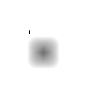
\begin{tikzpicture}
    % draw the shadow
    \foreach \x in {0,0.05,...,1} {
      \setlength{\shadowiter}{\boxshadowsize*\real{\x}}
      \fill[xshift=\boxshadowsize-1pt,yshift=-\boxshadowsize+1pt,
          black,opacity=0.04,rounded corners=\boxroundness]
          (\shadowiter,\shadowiter) rectangle +(\boxw-2\shadowiter,\boxh-2\shadowiter);
    }
    % draw the box border
    \filldraw[fill=\fillcolor,draw=\drawcolor,rounded corners=\boxroundness]
        (0,0) rectangle (\boxw,\boxh);
    % draw the content
    \node[xshift=\boxroundness,yshift=\boxroundness,inner sep=\innersep,outer sep=0pt,anchor=south west]
        at (0,0) {\usebox{\shadowblockbox}};
  \end{tikzpicture}
}

\newcommand\gitcmd[1]{%
%\begin{center}
%  \noindent\fcolorbox{white}{yellow!20}{%
%    \begin{minipage}{.7\textwidth}
%      \centering\Large
%      \texttt{#1}
%    \end{minipage}}
%\end{center}

\begin{center}
  \begin{shadowblock}{0.9\textwidth}{yellow!50}{black!50}{0pt}
  \centering\Large
  \texttt{#1}
  \end{shadowblock}
\end{center}
}

%\newsavebox{\framedtextbox}
%\newenvironment{framedtext}[1] % minipage width
%{\begin{lrbox}{\framedtextbox}\begin{minipage}{#1}\centering}
%{\end{minipage}\end{lrbox}
%  % put box in a tikz node, and draw the node.
%  \begin{tikzpicture}
%    \node [fill=gray!20,rounded corners] at (0,0) {\usebox{\framedtextbox}};
%  \end{tikzpicture}
%}
\newenvironment{framedtext}
{\begin{center}\begin{shadowblock}{0.7\textwidth}{gray!20}{red}{10pt}\ttfamily}
{\end{shadowblock}\end{center}}

\newcommand\surrounded[1]{
  \textless#1\textgreater
}

\newcommand\optionalSurrounded[1]{
  [\textless#1\textgreater]
}


\sybtitle{JavaScript Notes}
\sybauthor{孙延宾}
\sybdate{\today}

\begin{document}
\tt % I love Typewriter font.
%%%%%%%% the title page and toc %%%%%%%%%%
\pagestyle{header}
\sybmaketitle
\tableofcontents
\newpage

%%%%%%% the main content %%%%%%%%%
\pagestyle{main}
\setcounter{page}{1}

\part[JavaScript和DOM]{JavaScript和DOM}
\section[DOM是什么]{DOM是什么}
DOM(Document Object Model)是使用"JavaScript对象"来表示网页各个组成部分的方式。
网页被分解为一个个的node,最常用的是element nodes,attribute nodes和
text nodes三种,整个网页(the whole document)用document node来表示。

\section[获取页面元素]{获取页面元素}
获取页面元素有以下几种方式。
\subsection[Element ID]{Element ID}
\begin{javascriptcode}
  var widget = document.getElementById("widget");
  alert(widget);
\end{javascriptcode}

\subsection[Tag name]{Tag name}
\begin{javascriptcode}
  var pars = document.getElementsByTagName("p");
  for(var i = 0; i < pars.length; i++) {
    alert(pars[i]);
  }
\end{javascriptcode}

\subsection[Element name]{Element name}
\begin{javascriptcode}
  var widgetName = document.getElementsByName("widgetName")[0];
  alert(widgetName);
\end{javascriptcode}

\section[DOM node]{DOM node}
DOM将整个页面分解为node objects,所有的一切都是node object。
每个node都有三种属性:nodeType,nodeName,nodeValue。其中
nodeType用数字表示,如Node.ELEMENT\_NODE,nodeName用字符串表示,
如"H1"、"P"。

\subsection[Node之间的关系]{Node之间的关系}
所有的node都有下列属性:

\begin{itemize}
\item childNodes
\item firstChild
\item lastChild
\item nextSibling
\item previousSibling
\item parentNode
\end{itemize}

\subsection[获取node属性]{获取node属性}
第一种方式:通过node的".attributes"属性。

\begin{javascriptcode}
  <input type="text" name="widgetName" id="widget" />
  
  var output = '';
  var widget = document.getElementById("widget");
  var attrs = widget.attributes;
  for(var i = 0; i < attrs.length; i++) {
    output += attrs[i].name + '=' + attrs[i].value + '\n';
  }
  alert(output);
\end{javascriptcode}

第二种方法:getAttribute(name)

\begin{javascriptcode}
  var widget = document.getElementById('widget');
  alert(widget.getAttribute('type')); // display 'text'
  // or
  alert(widget.getAttributeNode('type')); // 打印node而不是其value
\end{javascriptcode}

当然,还可以预先判断某个属性是否存在:

\begin{javascriptcode}
  var isAttributeExists = elem.hasAttribute(attributeName);
\end{javascriptcode}

\subsection[修改node的属性]
改变属性值:

\begin{javascriptcode}
  <div>
    <img id="photo" src="cat.jpg" alt="My cat" />
  </div>

  var photo = document.getElementById('photo');
  var photoSrc = photo.getAttributeNode('src');
  var photoAlt = photo.getAttributeNode('alt');
  photoSrc.value = 'dog.jpg';
  photoAlt.value = 'My dog';
\end{javascriptcode}

增加属性:

\begin{javascriptcode}
  <div>
    <img id="photo" src="cat.jpg" alt="My cat" />
  </div>

  var photo = document.getElementById('photo');
  var width = document.createAttribute('width');
  width.value = 50;
  photo.setAttributeNode(width);
\end{javascriptcode}

快捷方式:

\begin{javascriptcode}
  // 如果name属性存在就修改其值,否则就增加name属性并设置其值为value
  elem.setAttribute(name, value);
\end{javascriptcode}

删除属性:

\begin{javascriptcode}
  //elem.removeAttribute(name);
  var photo = document.getElementById('photo');
  photo.setAttribute('width', 50);
  photo.removeAttribute('width');
\end{javascriptcode}


\subsection[修改node的值]{修改node的值}
修改node的值,只需修改node的nodeValue即可。

\begin{javascriptcode}
  <div id='welcome'> <p>Welcome to Widget.</p></div>
  var welcome = document.getElementById('welcome');
  welcome.firstChild.firstChild.nodeValue = 'Welcome U.';
\end{javascriptcode}

添加新的node:

\begin{javascriptcode}
  // 在尾部增加
  var welcome = document.getElementById('welcome');
  var horizRule = document.createElement('hr');
  welcome.appendChild(horizRule);
  // or
  // 在头部增加
  welcome.insertBefore(horizRule, welcome.firstChild);
\end{javascriptcode}

删除node:

\begin{javascriptcode}
  var welcome = document.getElementById('welcome');
  var horizRule = welcome.lastChild;
  welcome.removeChild(horizRule);
\end{javascriptcode}

替换node:

\begin{javascriptcode}
  var welcome = document.getElementById('welcome');
  var horizRule = welcome.lastChild;
  var newPar = document.createElement('p');
  newPar.appendChild(document.createTextNode('xxxxxx'));
  welcome.replaceChild(newPar, horizRule);
\end{javascriptcode}

移动node:

\begin{javascriptcode}
  <ul>
    <li id="widget1"><a href="superwidget.html">SuperWidget</a></li>
    <li id="widget2"><a href="megawidget.html">MegaWidget</a></li>
    <li id="widget3"><a href="wonderwidget.html">WonderWidget</a></li>
  </ul>
  // 只需将原来的node添加到需要的位置即可,旧的node自动删除,
  // 所以要想复制一个node就要使用createElement才行。
  var superWidget = document.getElementById("widget1");
  var ul = superWidget.parentNode;
  ul.appendChild(superWidget);
\end{javascriptcode}


\section[Prototype]{Prototype}
JavaScript的继承使用的是原型链(prototype chain)方式,原型链方式看似简单,
实则不然,理解原型链需从两方面进行:constructor模式、prototype模式。

\subsection[constructor mode]{constructor mode}
JavaScript 中没有类的概念,我们知道类是OOP中的"模型",那JS中如何定义模型呢?
答案是“构造函数”,在JS中,new关键词后面跟的是函数,构造函数。构造函数定义了
对象的模型,js中的任何对象都有constructor属性,该属性是对象到其构造函数的通道。
但是如果手动修改constructor属性,该通道也就被改变了,而有时修改构造函数是必须的
[见第\ref{sec:inherit}节],
所以通过该属性寻找构造函数是十分危险的事情。

\subsection[prototype mode]{prototype mode}
可以给构造函数增加"prototype"属性(函数也是对象哦!),其值为一个对象,以此来
达到对象的“继承”,这就是prototype mode。prototype属性只在函数中起作用。
另外需注意:

\emph{构造函数里的prototype对象是给其“实例”使用的!}

要想取得对象本身的prototype对象,则需要通过其constructor,

\begin{javascriptcode}
  // 构造函数与普通函数唯一的区别是首字母大写!
  function Foo() {};
  // 构造函数的prototype对象是给其“实例”使用的
  Foo.prototype = {
    foo:42
  };

  // 以Foo为模型,定义新的对象
  var obj = new Foo();
  // 对象的原型需要通过构造函数获得,而不是prototype属性
  var pt = obj.constructor.prototype; // 等于 {foo:42}
\end{javascriptcode}

容易造成迷惑的是函数的prototype属性及函数对象本身的prototype对象,

\begin{javascriptcode}
var pt = {
    bar: 42
};
function Bar() {};
// 函数的prototype属性,供其实例对象使用
Bar.prototype = pt;
alert(Bar.constructor === Function); // true
alert(Bar.constructor.prototype === Function.prototype); // true

// 注意:Object, Function, Array, Date都是函数(Math是对象)
\end{javascriptcode}

\section[变量声明、函数声明提升]{变量声明、函数声明提升}
这个绝对是JavaScript里面的奇葩:var表达式、函数声明被提升到当前
作用域的顶部。

名词解释:

声明(Declaration):\\
\begin{javascriptcode}
  var joe;
\end{javascriptcode}

初始化(Initialization):\\
\begin{javascriptcode}
  joe = 'plumber';
\end{javascriptcode}

示例:\\
\begin{javascriptcode}
  function f() {
    var a = 'a';
    // other code
    var b = 'b';
    // other code
    c();
    function c() {
      var aa = 'aa';
      // another code
      var bb = 'bb';
      // another code
    }
    // other code
  }
\end{javascriptcode}

等价于,

\begin{javascriptcode}
  function f() {
    var a, b; // 变量声明
    function c() {
      var aa, bb; // 变量声明
      aa = 'aa';
      // another code
      bb = 'bb';
      // another code
    }
    a = 'a';
    // other code
    b = 'b';
    // other code
    c();
    // other code
  }
\end{javascriptcode}

测试:alert输出时什么呢?\\
\begin{javascriptcode}
  var myvar = 'my value';
  (function () {
    alert(myvar);
    var myvar = 'local value';
  })();
\end{javascriptcode}

答案:undefined

函数声明也是一样的,所以可以在定义函数之前就使用函数!

\section[prototype.constructor]{prototype.constructor}
这绝对是个大坑!!!\label{sec:inherit}

\begin{javascriptcode}
  // 如果Foo是个空函数,即函数体中什么都没有,
  // 那么Foo实例的constructor就会是Object函数,
  // 这太坑爹了吧!
  function Foo() {foo:1};
  function Bar() {bar:1};
  Bar.prototype = new Foo();
  // 这一行是必须的,否则继承链就会紊乱,
  // 因为new新的实例时,新实例的constructor默认设置为
  // 构造函数的prototype.constructor,除非构造函数
  // 没有prototype属性,太坑爹了!
  var bar0 = new Bar();
  // bar0.constructor === Foo; // true!!!
  // 所以,修改构造函数的prototype属性时,后面跟的必定是
  // 修改prototype对象构造函数这一步!!!
  Bar.prototype.constructor = Bar;
  var bar = new Bar();
  // bar.constructor === Bar; // true
  
\end{javascriptcode}

\section[prototype mode详解]{prototype mode详解}
以下三种继承方式,其prototype chain是完全不同的。

\begin{javascriptcode}
  // Foo 构造函数
  function Foo() { foo1:1 };
  foo.prototype = { foo2:2 };

  // Bar 构造函数
  function Bar() { bar1:11 };

  // 这里填写继承关系,见下面三种继承方式

  var foo = Foo();
  var bar = Bar();
\end{javascriptcode}

\subsection[父子关系]{父子关系}
第一种继承方式:父子关系

\begin{javascriptcode}
  Bar.prototype = new Foo();
  // 这是必须的!
  Bar.prototype.constructor = Bar;
\end{javascriptcode}

继承链:\\
bar\\
=> Foo的实例(即new Foo())\\
=> Foo.prototype对象\\
=> Object.prototype对象(即{},空对象)\\
foo与bar是父子关系。这是最常见的继承方式。

\subsection[兄弟关系]{兄弟关系}
第二种继承方式:兄弟关系

\begin{javascriptcode}
  Bar.prototype = Foo.prototype;
\end{javascriptcode}

继承链:\\
bar\\
=> Foo.prototype对象\\
=> Object.prototype对象(即{},空对象)\\
foo\\
=> Foo.prototype对象\\
=> Object.prototype对象(即{},空对象)\\
foo与bar是兄弟关系。

\subsection[陌生关系]{陌生关系}
第三种继承方式:陌生关系

\begin{javascriptcode}
  Bar.prototype = Foo;
\end{javascriptcode}

继承链:\\
bar\\
=> Foo对象(函数也是对象)\\
=> Foo.constructor.prototype(即Function.prototype)\\
foo\\
=> Foo.prototype\\
=> Object.prototype对象(即{},空对象)\\
Foo的实例与Bar的实例没有关系。

\end{document}